\section{Overview}
This report contains figures related to the calibration
process of autocorrelator data from Odin-SMR.\\
\newline
Topics examined are:\\
\newline
Calibration of sky signals\\
The statistics of calibrated sky signals seems to be fine
except that mean and median spectra deviates from 0 K
(overestimation of sky signal with up to\(\sim\)0.3 K).
The reason for this should most likely be due to that
the gain varies (for some reason) in a systematic non-linear manner
in such a way that linear interpolation
of reference signals give rise to a systematic error
in the calibration procedure.\\
\newline
Spectral feature in high altitude spectrum\\
The spectral features seen in high altitude spectra are
examined. Spectra are sorted in temperature bins
using hotload temperature as a reference.
It is shown that the phase of the signal seen in high
altitude spectra varies with temperature.
%Thus it seems possible to remove this spectral
%feature from spectra in the calibration procedure by something like:\\
%*first perform the ``standard'' calibration
%*create a table with results from high 
%altitude measurements and e.g. hotload temperatures
%*Perform a second calibration
%\\
\clearpage
\newpage

\section{Calibration of sky signals}
In this section results from the calibration of sky signals
from AC2 (stratospheric mode 1) and AC1 (stratospheric mode 2)
are shown. The shape and statistics of calibrated skysignal
spectra from several orbits are explored.  

The calibration of sky signals is done by:
\begin{equation}
\label{eq:skysig}
T^{'}_{sky}=\frac{c_{sky}-c^{'}_{sky}}{g^{'}}+T_{sky}\approx(\frac{g}{g^{'}}-1)T_{sys},
\end{equation}
where \(T^{'}_{sky}\) is the estimation of the brightness temperature
of the sky signal, \(c_{sky}\approx g(T_{sys}+T_{sky})\approx gT_{sys}\) is the measured sky signal,
 \(c^{'}_{sky}\) is the reference estimated sky signal
which is retrieved using linear interpolation w.r.t. time using
the measured skysignals around the target \(c_{sky}\),   
\(g\) is the true
gain, and \(g^{'}\) is the estimated gain, \(T_{sys}\) is the system
noise temperature. 

Equation~\ref{eq:skysig} gives that, even if the gain varies
linearly with time and that we can estimate \(g^{'}=g+\Delta g\) with
an error \(\Delta g\) that is gaussian distributed and has zero mean,
we would expect the average sky signal spectrum to deviate from 
0 K. The simple reason for this is that a positive and negative
error in gain will not totally cancel out, i.e. 
\(\frac{g}{g+\Delta g} \neq \frac{g}{g-\Delta g}\).    
However, in this case the median spectrum would be very close to
0 K.
In this section it is shown that both mean and median of calibrated
skysignal spectra deviates from 0 K.


\clearpage
\newpage

\subsection{AC2}
\begin{figure}[!t]
\centering
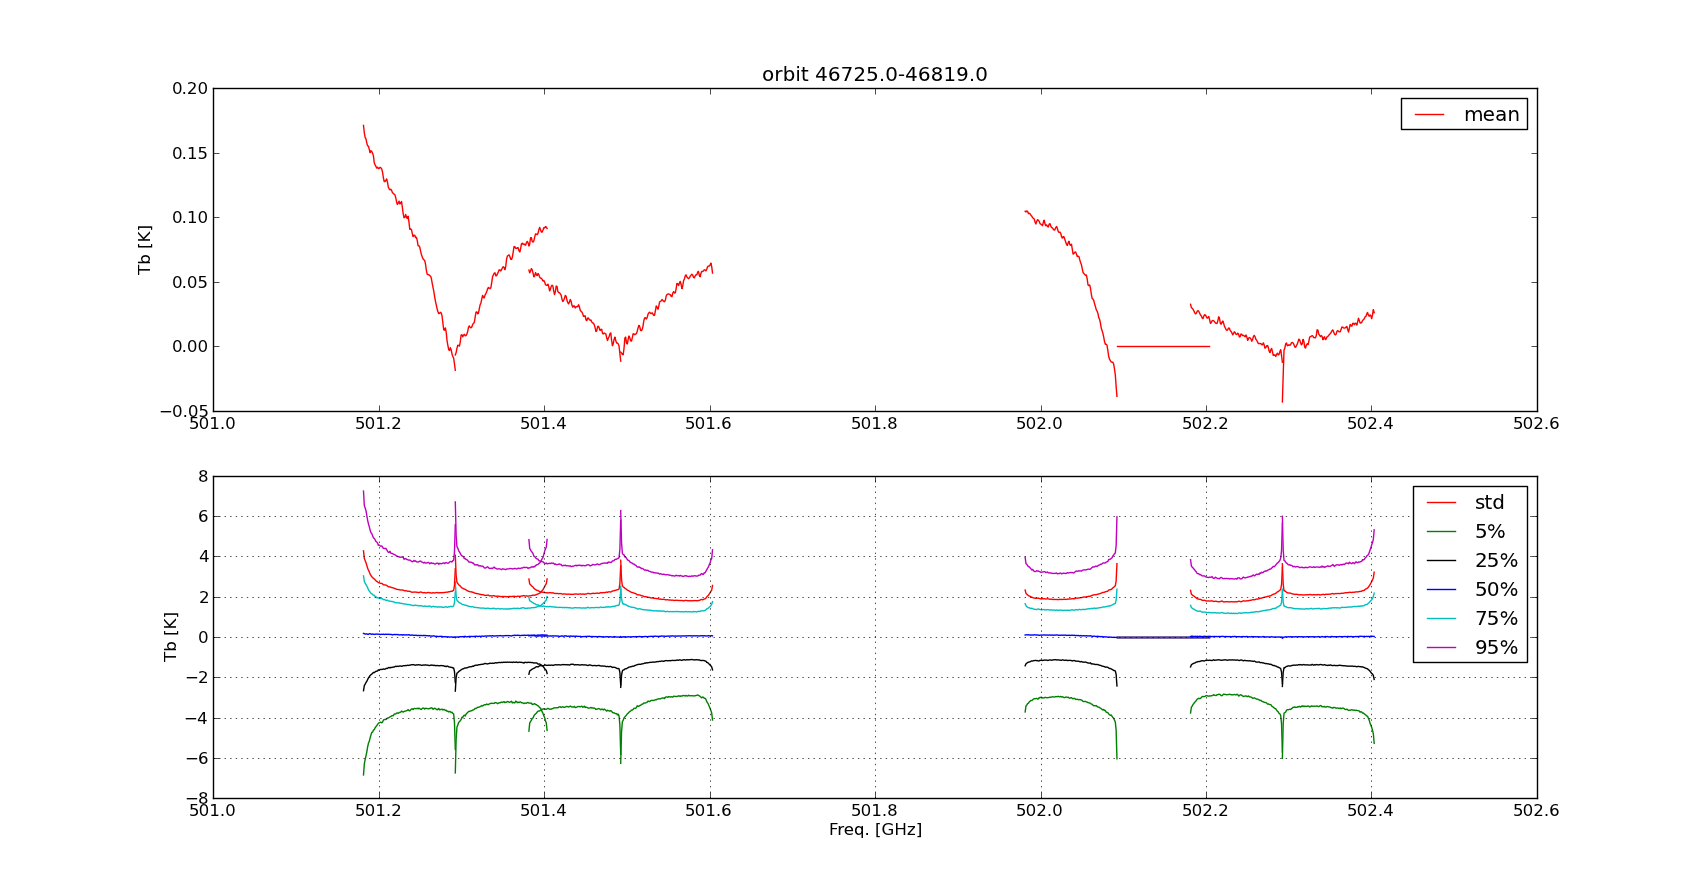
\includegraphics[scale=0.35]{ac2skycal1.png}\\
\caption{The upper panel shows a mean spectrum of calibrated
skysignals from AC2 stratospheric mode 1. 
The lower panel show a standard deviation spectrum
and percentiles spectra.}
\label{fig:study3ac2a}
\end{figure}

\begin{figure}[!t]
\centering
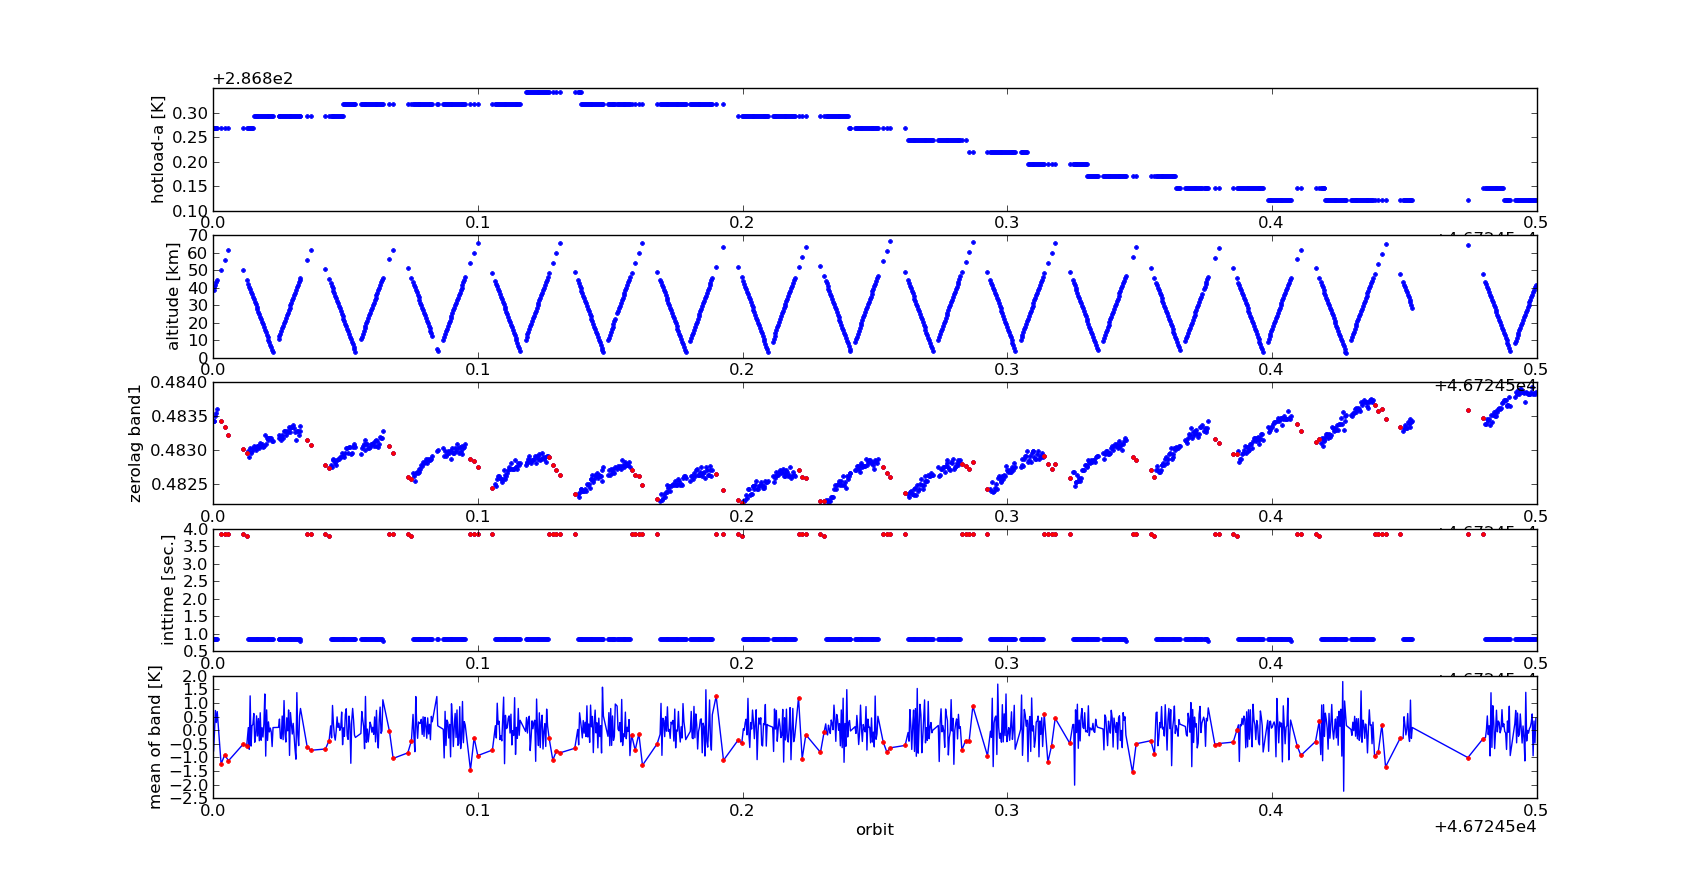
\includegraphics[scale=0.35]{ac2skycal2.png}\\
\caption{Time series of various data from part of an orbit.
The upper (first) panel shows hotload temperatures.
The second panel shows tangent altitudes.
The third panel shows zerolags of skysignals for band 1 of AC2.
The fourth panel shows integration times.
The lower panel shows band 1 average calibrated brightness temperatues.}
\label{fig:study3ac2b}
\end{figure}


The upper panel of Figure~\ref{fig:study3ac2a} shows a mean spectrum
of calibrated sky signals from several orbits. It can clearly be seen
that this spectrum deviates from 0 K (approximately the true brightness 
temperature of the sky signal).
The lower panel shows some additional statistics.
The standard deviation of the spectrum is around 2 K,
which agrees well with the expected theoretical noise level
(\(\Delta T =T_{sys}/\sqrt{B*\tau} \approx 3000 K / \sqrt{2MHz*1s}=2.1 K\)).
The percentiles (for example the 25 and 75) are fairly evenly
displaced from the 50\% percentile (median),
which means that the errors are at least close to gaussian
distributed.  
The median has the same pattern as the mean (which is hard to see
due to the scale).

The reason for the median deviation from 0 K is most likely due to 
some systematic gain variations, i.e. the gain does not vary
completely linearly with time between three sky signals
measurements.

%Equation~\ref{eq:skysig} gives that, even if the gain varies
%linearly with time and that we can estimate \(g^{'}=g+\Delta g\) with
%an error \(\Delta g\) that is gaussian distributed and has zero mean,
%we would expect the average sky signal spectrum to deviate from 
%zero. The simple reason for this is that a positive and negative
%error in gain will not totally cancel out, i.e. 
%\(\frac{g}{g+\Delta g} \neq \frac{g}{g-\Delta g}\).
%However, since \(\Delta g\) in general is very small this
%does not explain the shape of the median spectrum in Figure~\ref{fig:ac2a}. 

Figure~\ref{fig:study3ac2b} show time series of various data from 
part of an orbit.
The middle panel shows the variation of zerolags for band 1
of AC2 (the variation of zerolags from other bands looks similiar).
On a short time scale (over one scan down and up) the zerolags increases
until the 4 seconds integration time starts. Then zerolags decreases
during the period with four seconds integration times. 
It seems that for the time period when zerolags increases
the increase is not totally linear in time.

This means that on average we probably make a systematic
error or underestimation of \(c^{'}_{sky}\) in the calibration
procedure, which means that we overestimate \(T^{'}_{sky}\)
(see Equation~\ref{eq:skysig}).
To overcome this problem a possible solution would be to use a weighted
quadratic interpolation as we have earlier discussed.

\clearpage
\newpage
\subsection{AC1}

\begin{figure}[!t]
\centering
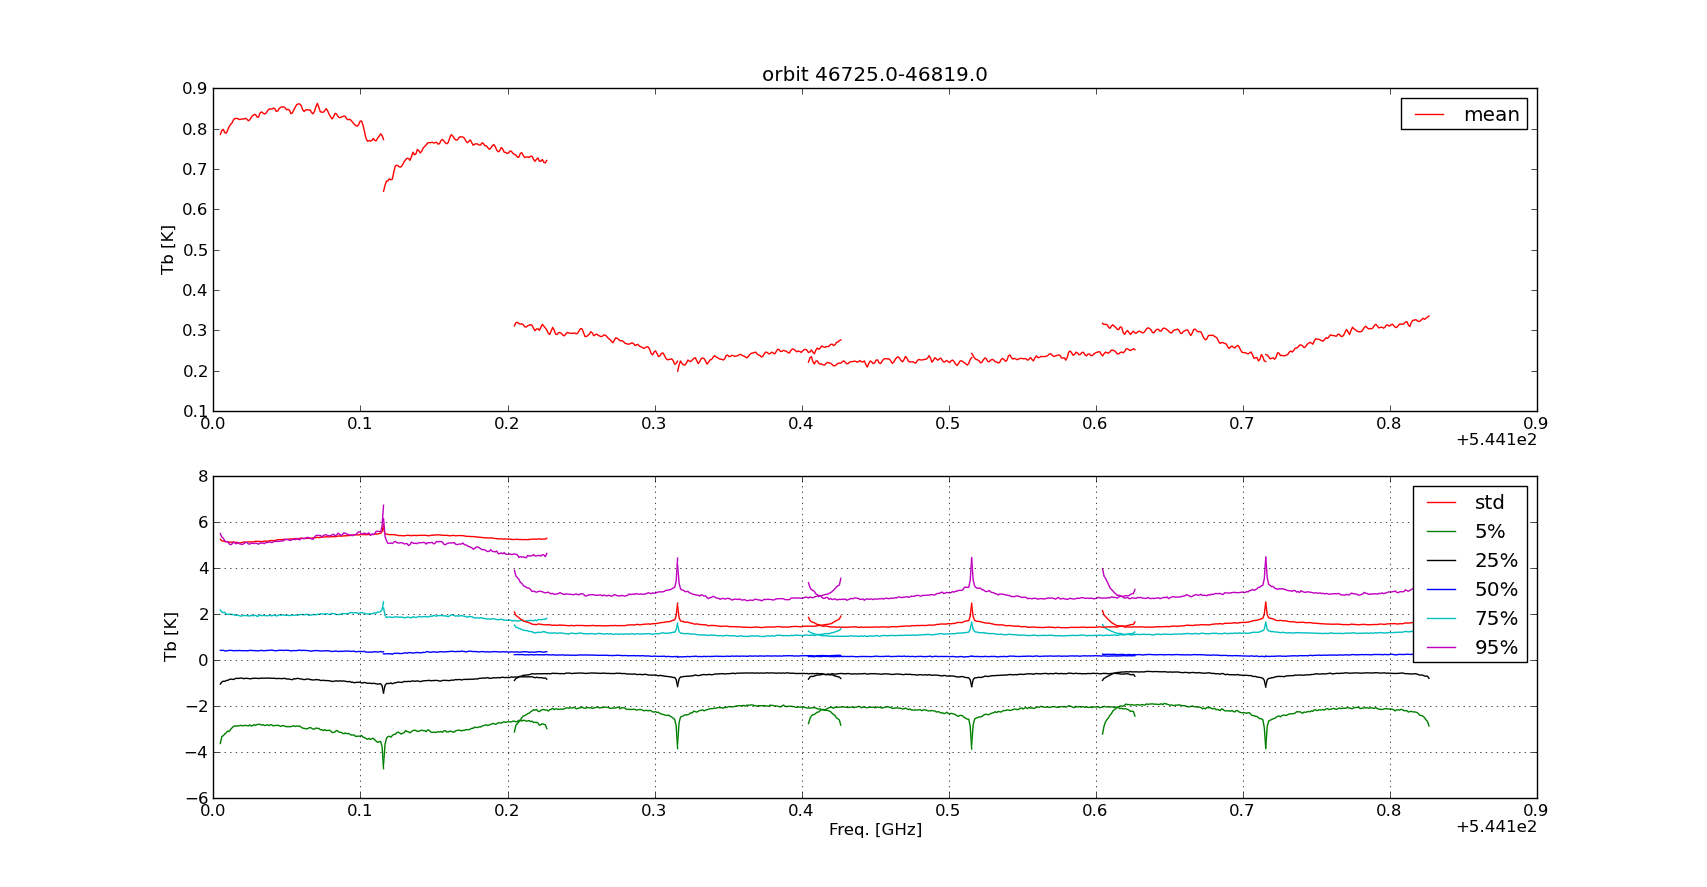
\includegraphics[scale=0.35]{ac1skycal1.png}\\
\caption{The upper panel shows a mean spectrum of calibrated
skysignals from AC1 stratospheric mode 2. 
The lower panel show a standard deviation spectrum
and percentiles spectra.}
\label{fig:study3ac1a}
\end{figure}

\begin{figure}[!t]
\centering
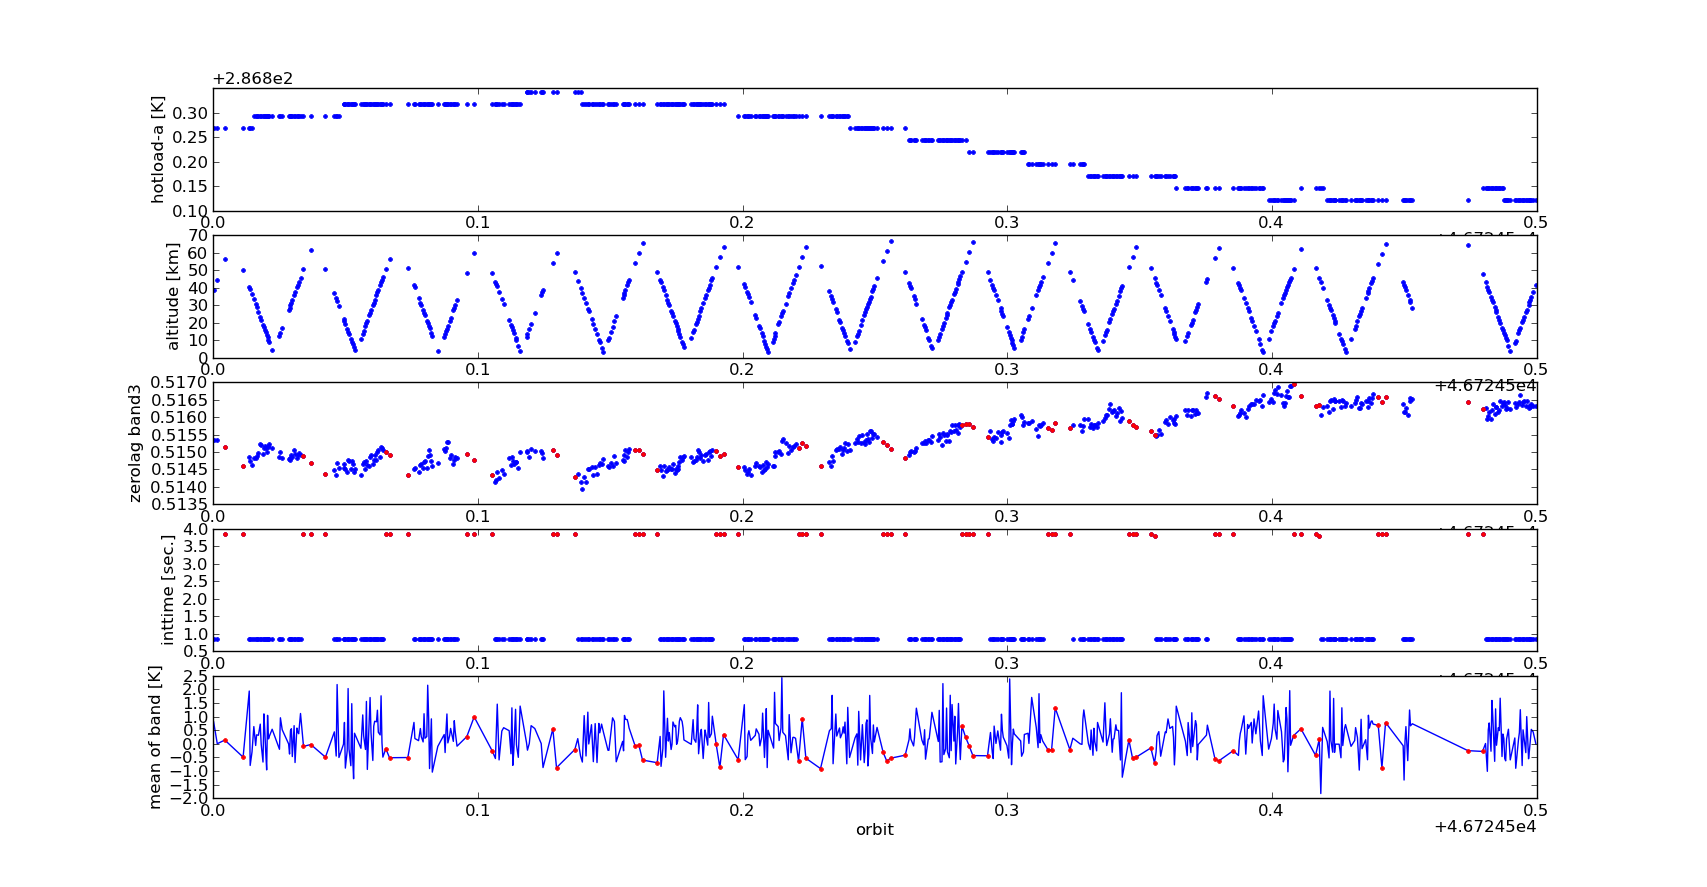
\includegraphics[scale=0.35]{ac1skycal2.png}\\
\caption{Time series of various data from part of an orbit.
The upper (first) panel shows hotload temperatures.
The second panel shows tangent altitudes.
The third panel shows zerolags of skysignals for band 3 of AC1.
The fourth panel shows integration times.
The lower panel shows band 1 average calibrated brightness temperatues.}
\label{fig:study3ac1b}
\end{figure}

 
Figures~\ref{fig:study3ac1a} and~\ref{fig:study3ac1b} show corresponding
data as Figures~\ref{fig:study3ac2a} and~\ref{fig:study3ac2b}
but for AC1 (stratospheric mode 2).
The results look very similiar for AC1 as for AC2.
The statistics of calibrated sky signals looks as expected
except that mean and median values deviates from 0 K
with around 0.25 K (Figure~\ref{fig:study3ac1a}),
except the two problematic bands in the lower part of the
spectrum.
Similiar pattern of short time scale variations in zerolag
as for AC2 is obsereved (Figure~\ref{fig:study3ac1b}).


\clearpage
\newpage
\section{High altitude spectra}   
\begin{figure}[!t]
\centering
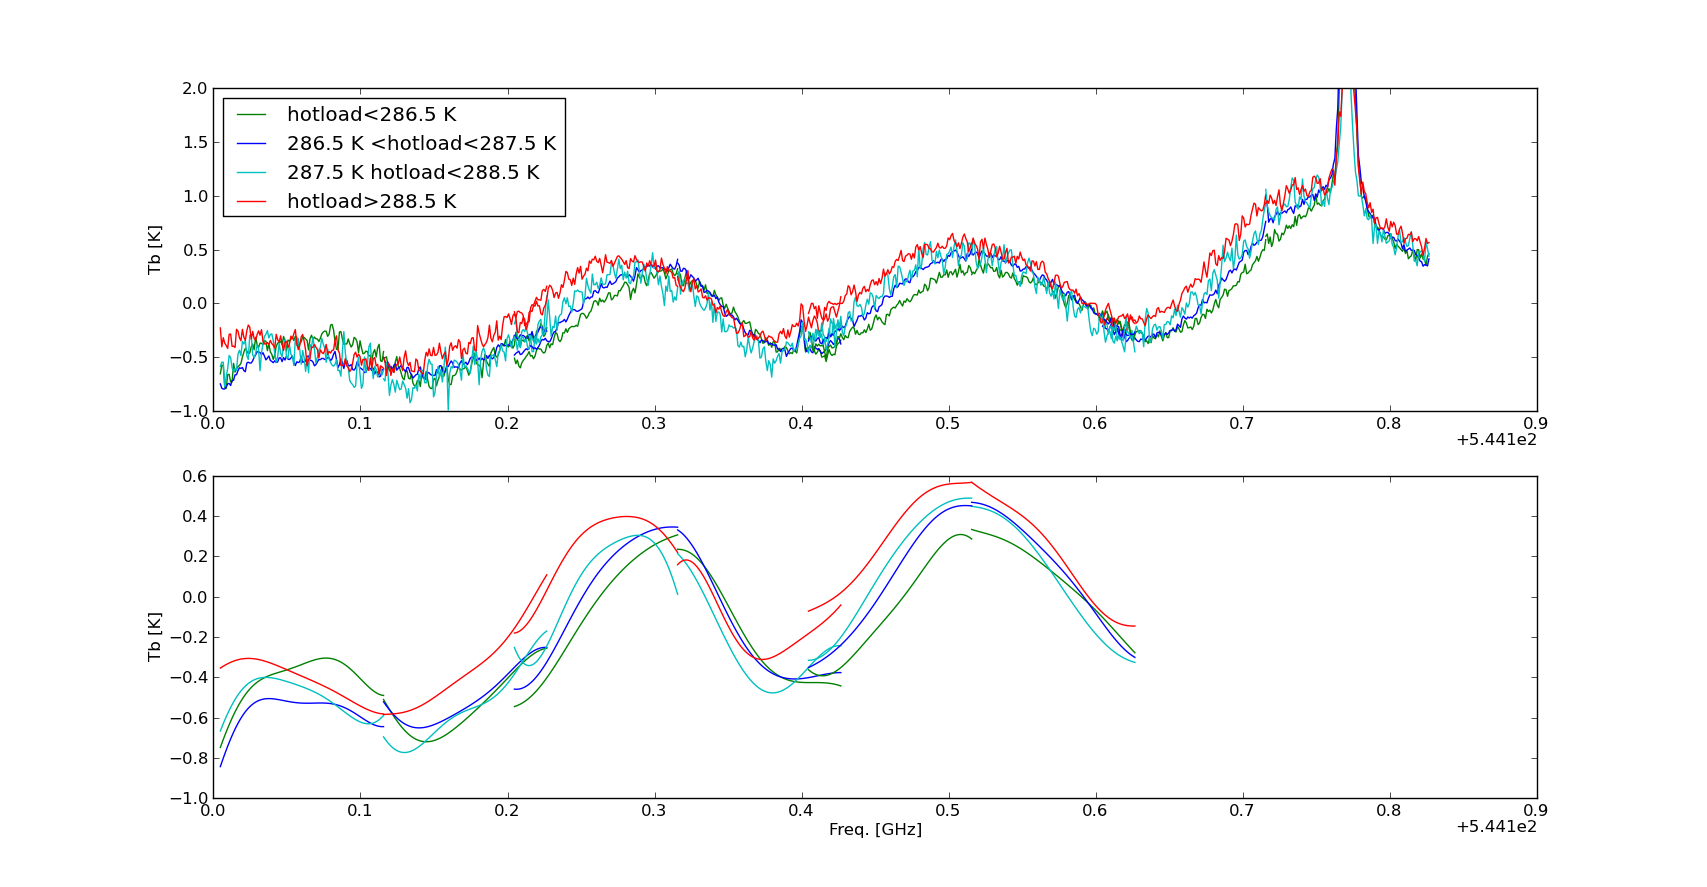
\includegraphics[scale=0.35]{ac1highalt.png}\\
\caption{The upper panel show median of high altitude (60-120 km)
spectra for different temperatures for AC1 stratospheric mode 2.
The lower panel shows fits to spectra in the upper panel.}
\label{fig:study3ac1c}
\end{figure}

\begin{figure}[!t]
\centering
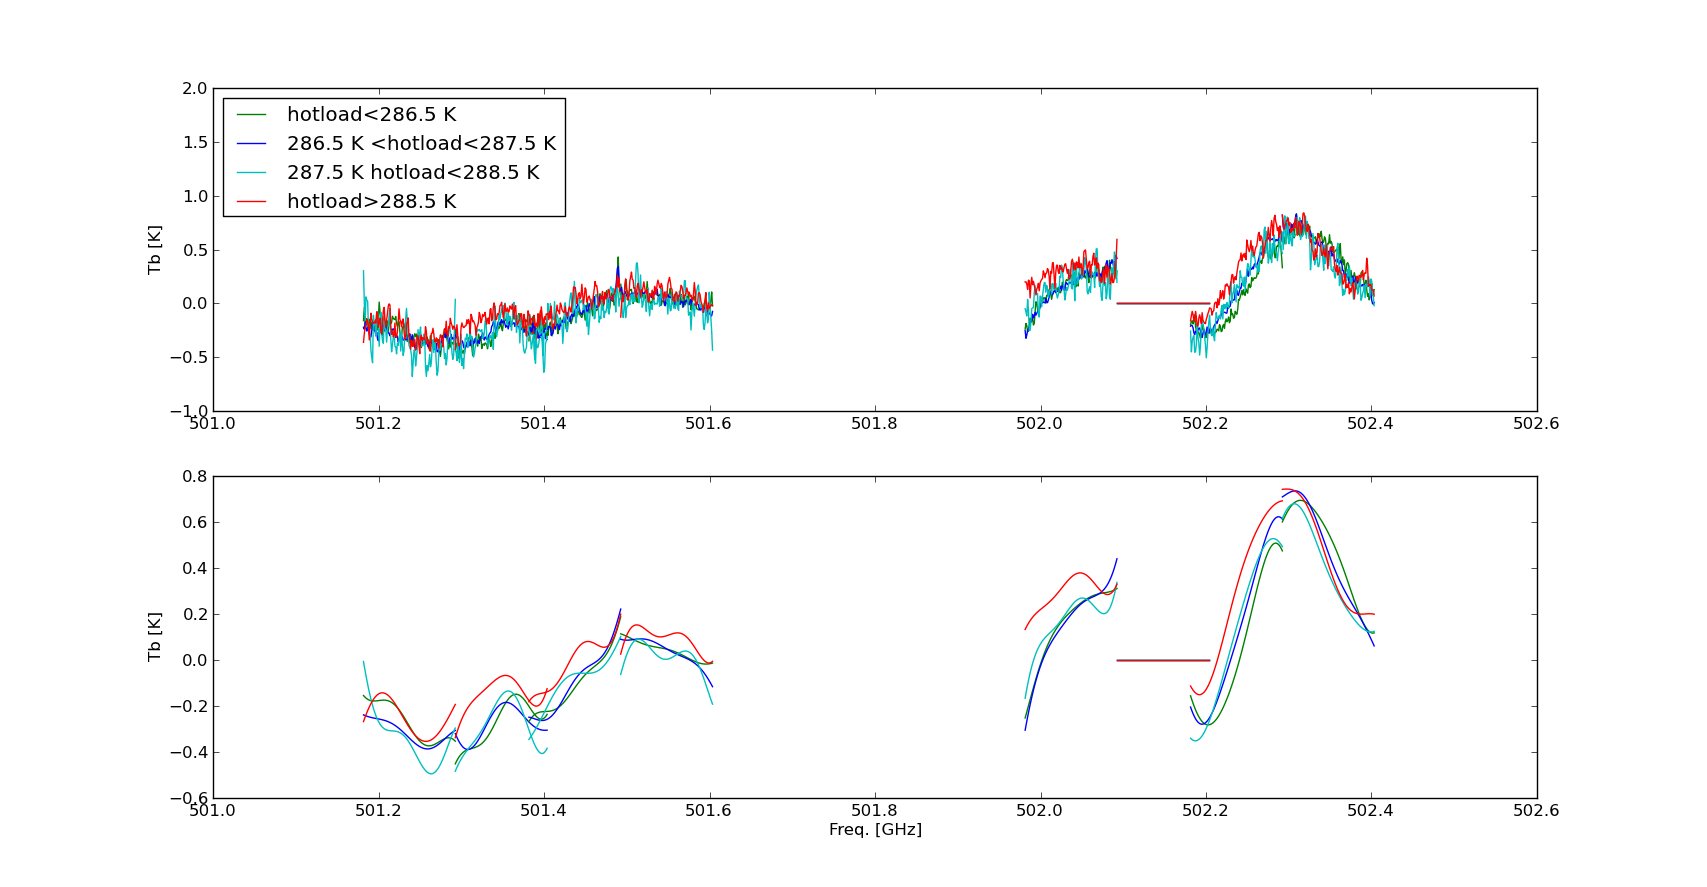
\includegraphics[scale=0.35]{ac2highalt.png}\\
\caption{The upper panel show median of high altitude (60-120 km)
spectra for different temperatures for AC2 stratospheric mode 1.
The lower panel shows fits to spectra in the upper panel.}
\label{fig:study3ac2c}
\end{figure}


In this section high altitude spectra from AC1 and AC2 are explored.
We know from earlier studies that these spectra contains
spectral features even though we do not expect this.
This spectral features should come from that either the sky signal
or the target signal is perturbed. Most likely it comes from ripple on the
sky signal. Regardless where it comes from, it should be possible to remove
this spectral feature in the calibration process. Although, the way to
properly remove it depends on where it comes from.

However, in this section we look at the temperature dependence
of the spectral features. Figures~\ref{fig:study3ac1c} and~\ref{fig:study3ac2c}
shows median of calibrated high altitude measurements from around 
200 orbits from 2009-08-24 to 2009-09-24. 
The data is sorted in temperature bins using the hotload temperature
as reference temperature.   
Figure~\ref{fig:study3ac1c} shows that the phase of the signal seen in AC1 
high altitude measurements varies with temperature.
This effect can also be seen in Figure~\ref{fig:study3ac2c} for AC2
although it is not so clear as for AC1.






